\section{Introduction}
\label{sec:intro}
\IEEEPARstart{V}{ideo} restoration and enhancement aim to improve visual information acquired under imperfect imaging, transmission, and generation conditions. Limited spatial resolution, sensor noise, motion blur, compression, and adverse illumination can obscure both the appearance of a scene and its evolution over time. The problem extends beyond natural RGB video to faces, underwater scenes, infrared imaging, high-dynamic-range content, and AI-generated video. Across these settings, a useful reconstruction must recover detail while preserving the structures and events represented by the input.

Temporal redundancy distinguishes video restoration from its image counterpart. Neighboring frames can reveal complementary texture, compensate for occlusion, and constrain motion, enabling alignment, propagation, recurrence, and attention to improve reconstruction~\cite{vrsurvey,realbasicvsr}. However, information lost across an entire sequence remains difficult to recover. Under severe degradation, minimizing pixel-wise error often favors averaged, oversmoothed predictions. Perceptual and adversarial objectives address this limitation by encouraging realistic appearance. Diffusion models offer a further route through expressive, reusable image and video priors~\cite{ddpm,ldm,svd,wan}. Their success has motivated methods for real-world video super-resolution (VSR), generic restoration, and specialized enhancement~\cite{upscale,stablevsr,seedvr,undive}.

The use of generative priors changes the central restoration problem. A detailed frame can contain plausible texture that differs from the underlying scene, and independently synthesized textures can vary across frames even when the scene does not. Conversely, a temporally smooth reconstruction may preserve an incorrect face or suppress genuine motion. Diffusion-based video restoration consequently involves three closely related objectives: \emph{fidelity} to the observed scene, \emph{perceptual quality} of the reconstructed content, and \emph{temporal consistency} of appearance, geometry, identity, and motion. The published examples in Fig.~\ref{fig:tradeoff} make these distinctions visible. These objectives are not always aligned. Improving perceptual quality may increase reconstruction error, as described by the perception–distortion tradeoff. In video, generated details may also vary across frames, introducing flicker and temporal inconsistency. The central challenge is therefore to balance perceptual quality, fidelity, and temporal consistency.

\begin{figure*}[t]
\centering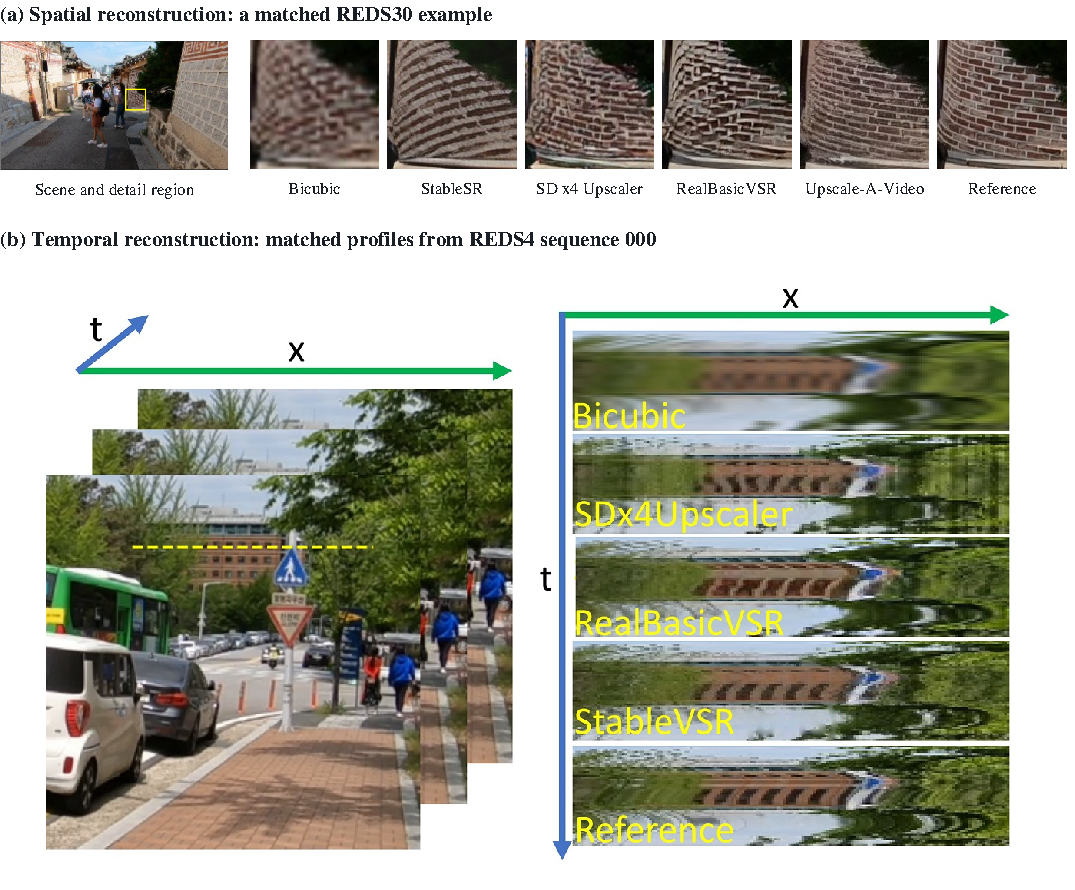
\includegraphics[width=\textwidth]{figures/tradeoff.pdf}
\caption{Published visual comparisons of spatial and temporal reconstruction. (a) Matched brick-wall crops from Upscale-A-Video~\cite{upscale}, Fig.~4, on REDS30: detail sharpness and agreement with the reference structure are different properties. The yellow box identifies the compared region. (b) Temporal profiles from StableVSR~\cite{stablevsr}, Fig.~6, on REDS4 sequence 000. Each profile stacks the same image row over time; horizontal position is $x$ and time runs downward. Irregular trajectories expose temporal artifacts.}
\label{fig:tradeoff}
\end{figure*}

Rapid changes in foundation models also complicate comparisons. Image diffusion models and video diffusion transformers differ in pretraining data, motion priors, model capacity, latent compression, and computational requirements. Restoration methods further vary in supervision, degradation simulation, temporal context, guidance, and sampling steps. A gain obtained with a stronger backbone can therefore reflect both a better prior and a better restoration mechanism. Meanwhile, one-step and streaming methods introduce new questions about first-frame latency, future-frame access, cache state, and the cost of encoding and decoding.

Evaluation must accommodate these changes. Reference-based distortion metrics measure agreement with a target, perceptual metrics assess appearance similarity, and no-reference predictors estimate viewing quality. None alone describes whether generated detail is faithful and temporally stable. Recent subjective evaluation of diffusion-based VSR shows that metric performance depends on the restoration method, source content, and aggregation protocol~\cite{metric}. Together with uneven task coverage, these issues motivate a survey that connects method design, application requirements, and evaluation.

Existing surveys provide complementary perspectives on this field. Li et al.~\cite{irsurvey} review diffusion-based image restoration through supervised and zero-shot formulations, conditioning strategies, and blind or real-world degradation. Jiang et al.~\cite{aiosurvey} organize all-in-one image restoration by network design, learning strategies, and techniques. These perspectives explain how restoration models acquire generality, but video additionally requires motion-aware processing and persistent content across frames. Xing et al.~\cite{videodiffsurvey} survey video diffusion models across generation, editing, and understanding. Their broad generative perspective provides foundations for temporal architectures and conditioning. Rota et al.~\cite{vrsurvey} review video restoration architectures, loss functions, and benchmarks, providing a detailed account of temporal information use. Building on these foundations, the present survey centers the interaction between diffusion priors and video reconstruction. Table~\ref{tab:surveys} summarizes the relationship between these lines of work.

\begin{table*}[t]
\caption{Representative surveys related to diffusion-based video restoration and enhancement.}
\label{tab:surveys}\centering\footnotesize
\begin{tabularx}{\textwidth}{@{}p{0.23\textwidth}YYY@{}}\toprule
Survey & Main focus & Principal organizing dimensions & Relation to video restoration \\\midrule
Diffusion image restoration~\cite{irsurvey} & Image reconstruction with diffusion models & Supervision, conditioning, generation space, real-world degradation & Establishes prior adaptation and inverse-problem formulations \\
All-in-one image restoration~\cite{aiosurvey} & Unified restoration across degradations & Architectures, learning, prompts, experts, multimodal and agentic systems & Motivates multi-task models and adaptive restoration systems \\
Video diffusion~\cite{videodiffsurvey} & Generation, editing, and video understanding & Generative architectures, conditions, applications & Provides spatiotemporal priors and includes restoration applications \\
Deep video restoration~\cite{vrsurvey} & Learning-based video reconstruction & Architecture, motion handling, losses, datasets & Establishes temporal modeling and task-specific evaluation \\
This survey & Diffusion-based video restoration and enhancement & Priors, conditioning, temporal mechanisms, tasks, efficiency, evaluation & Connects generative detail to source fidelity and temporal consistency \\\bottomrule
\end{tabularx}
\end{table*}

This survey covers methods that use diffusion, score-based, or related flow priors to restore a video, which spans spatial and spatiotemporal super-resolution, single and mixed degradation removal, domain-specific enhancement, and restoration of generated video. Our main contributions are as follows:
\begin{itemize}
\item We develop a unified taxonomy spanning degradation assumptions, learning strategies, prior sources, conditioning, temporal modeling, inference efficiency, and system organization.
\item We analyze how noise coupling, correspondence, propagation, attention, memory, and decoding connect generated detail to the input sequence, and compare the strengths and limitations of representative approaches.
\item We review restoration tasks across natural video and specialized domains, relating their imaging characteristics and temporal requirements to suitable generative models.
\item We examine datasets and evaluation metrics, discuss fair comparisons across heterogeneous backbones, and identify research directions in quality control, efficient long-video processing, and generalization.
\end{itemize}

Section~\ref{sec:formulation} introduces the background and problem formulation. Section~\ref{sec:methodology} reviews generative priors, conditioning, temporal modeling, learning strategies, and efficient inference. Section~\ref{sec:tasks} relates these mechanisms to restoration tasks and application domains. Section~\ref{sec:evaluation} discusses datasets, quality assessment, and fair comparisons, and Section~\ref{sec:outlook} identifies challenges and future directions.

\begin{figure*}[t]
\centering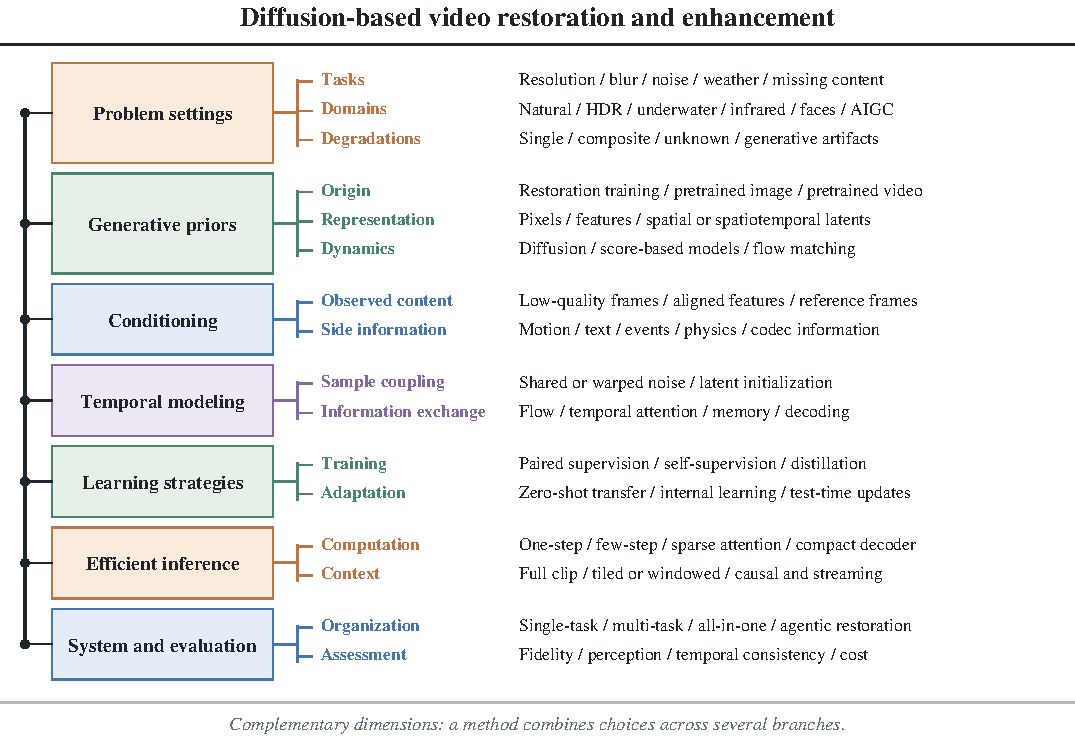
\includegraphics[width=\textwidth]{figures/taxonomy.pdf}
\caption{Taxonomy and organization of diffusion-based video restoration and enhancement. The classification connects task and degradation characteristics with generative priors, learning strategies, conditioning, temporal modeling, and inference.}
\label{fig:taxonomy}
\end{figure*}
